\chapter{Spoken Language Assessment} \label{chap:graders}

The three types of models under investigation are: text-based, feature-based, and audio-based models. Each grader has its own architecture, with different number of layers, neurons, activation functions, and dropout rates. The dropout rate is the proportion of neurons that are randomly set to zero during training, which helps prevent overfitting. Table \ref{activation functions} defines the types of activation functions under consideration, where $\alpha$ is a small constant ($<<1$) that allows a small gradient when the unit is not active.

\begin{table}[H]
    \centering
    \begin{tabular}{|c|c|}
        \hline
        \textbf{Activation Function}                                                             & \textbf{Definition}                     \\ \hline
        Rectified Linear Unit (ReLU) \nomenclature[Z]{ReLU}{Rectified Linear Unit}               & $f(x) = \max(0, x)$                     \\ \hline
        Leaky Rectified Linear Unit (LReLU) \nomenclature[Z]{LReLU}{Leaky Rectified Linear Unit} & $f(x) = \begin{cases}
                                                                                                                   x,        & \text{if } x > 0    \\
                                                                                                                   \alpha x, & \text{if } x \leq 0
                                                                                                               \end{cases}$ \\ \hline
    \end{tabular}
    \caption{Activation functions under consideration}
    \label{activation functions}
\end{table}

Each grader also have its own model type - it could be a deep neural network (DNN) \nomenclature[Z]{DNN}{Deep Neural Network} or a deep density network (DDN). A DNN directly outputs the score from the input vector, using mean squared error (MSE) \nomenclature[Z]{MSE}{Mean Squared Error} loss function. A DDN, on the other hand, predicts the score from the input vector using a Gaussian distribution, outputting the mean ($\mu$) \nomenclature[A]{$\mu$}{Mean} and the standard deviation ($\sigma$) \nomenclature[A]{$\sigma$}{Standard deviation}. It uses negative log-likelihood for multivariate Gaussian (NLL) \nomenclature[Z]{NLL}{Negative Log-Likelihood} loss function.

The formula for the MSE and NLL loss functions are given by:
\begin{equation} \label{eq:mse}
    \text{MSE} = \frac{1}{N} \sum_{i=1}^{N} (y_i - \hat{y}_i)^2
\end{equation}
\begin{equation} \label{eq:nll}
    \text{NLL} = -\frac{1}{N} \sum_{i=1}^{N} \left( \log(\sigma_i^2) + \frac{(y_i - \mu_i)^2}{(2\sigma_i^2 + \epsilon)} \right)
\end{equation}
where $N$ is the number of samples, $y_i$ is the true score,  $\hat{y}_i$ is the predicted score, and $\epsilon = 1\times10^{-8}$ is a small constant to prevent division by zero.

The result would then be passed through linear calibration with the output result shown in equation \ref{eq:calibration}. The calibration is done using a linear regression model, which is trained to minimize the MSE between the predicted and true score. The linear regression model outputs two parameters: the slope ($m$) \nomenclature[A]{$m$}{Slope} and the intercept ($c$) \nomenclature[A]{$c$}{Intercept}. The calibrated score is then calculated using the formula:

\begin{equation}
    \hat{y}_{\text{calibrated}} = m*\hat{y}_{\text{uncalibrated}} + c
    \label{eq:calibration}
\end{equation}

Each grader also has its own way to process the input data to the intermediate vector $\hat{x}$. The following sections describe the architecture of each model in detail.

\section{Text-based Model}
Figure \ref{fig:text} shows the architecture of the text-based model. The BERT processing begins with text transcript extracted by WHISPER automatic speech recognition (ASR) from the candidate's audio. Each sample is fed through the BERT tokenizer \nomenclature[Z]{BERT}{Bidirectional Encoder Representations from Transformers}, which converts the text into a sequence of independent tokens ($\mathcal{T}$). $\mathcal{T}$ is then passed through the BERT encoder, creating contextualized embeddings for the tokens ($\mathcal{C}$), which takes into account the surrounding tokens. $\mathcal{C}$ is further passed through four independent attention mechanisms. Their outputs, each of 768 dimensions, are concatenated to form the 3072-dimensional token embeddings $\hat{x}$.

The token embeddings $\hat{x}$ is then passed through a fully connected DNN with 2 hidden layers, using the ReLU activation function. Each layer is labelled with a red box, with the red number indicating the change in dimension after each layer. The output is a single scalar indicated the predicted score.

\begin{figure}[H]
    \centering
    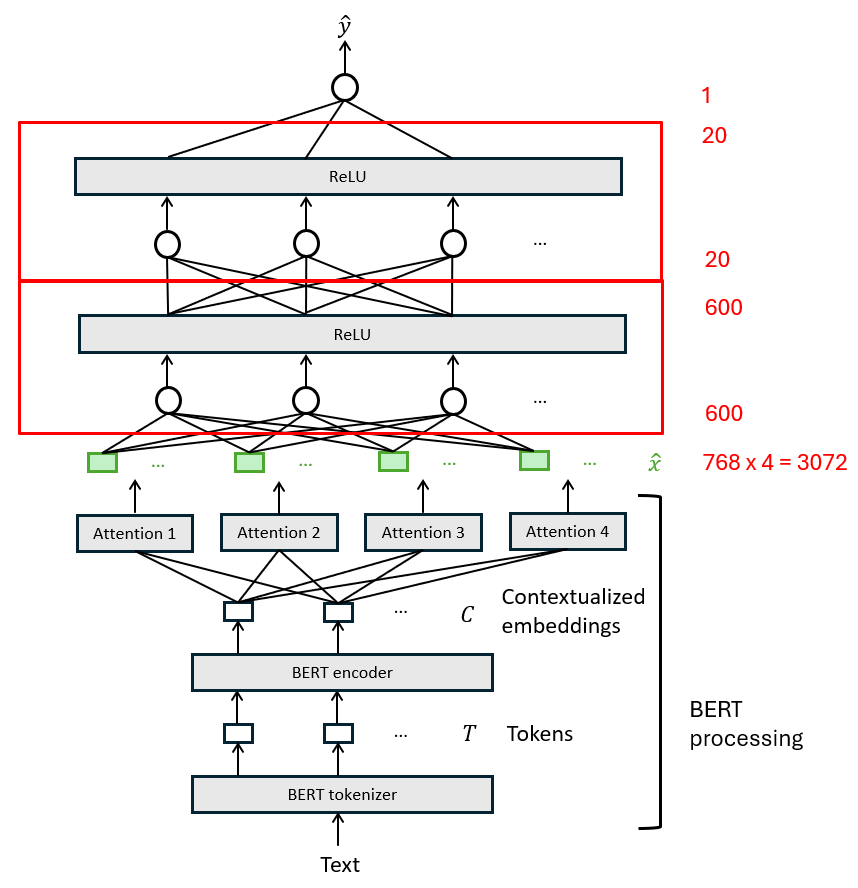
\includegraphics[width=0.7\textwidth]{text.png}
    \caption{Text-based model architecture}
    \label{fig:text}
\end{figure}

\section{Feature-based Model}
Figure \ref{fig:feature} shows the architecture of the feature-based model. The speech data have been extracted to produce a 356-dimensional vector using a custom extractor described in \cite{feature}. The features include statistics of: word level, phone duration, rhythm, fluency, and frequency \cite{graders}, with the full list of features detailed in \cite{feature}'s appendix.

The feature vector $\hat{x}$ is then passed through a fully connected DDN with 3 hidden layers. LReLU with $\alpha = 0.01$ is used as the activation function, and the dropout rate is set to 0.5. The output includes both $\mu$ and $\log(\sigma)$ of the predicted score Gaussian distribution. Similarly, the red box and red number indicated the layers and the dimension change.

\begin{figure}[H]
    \centering
    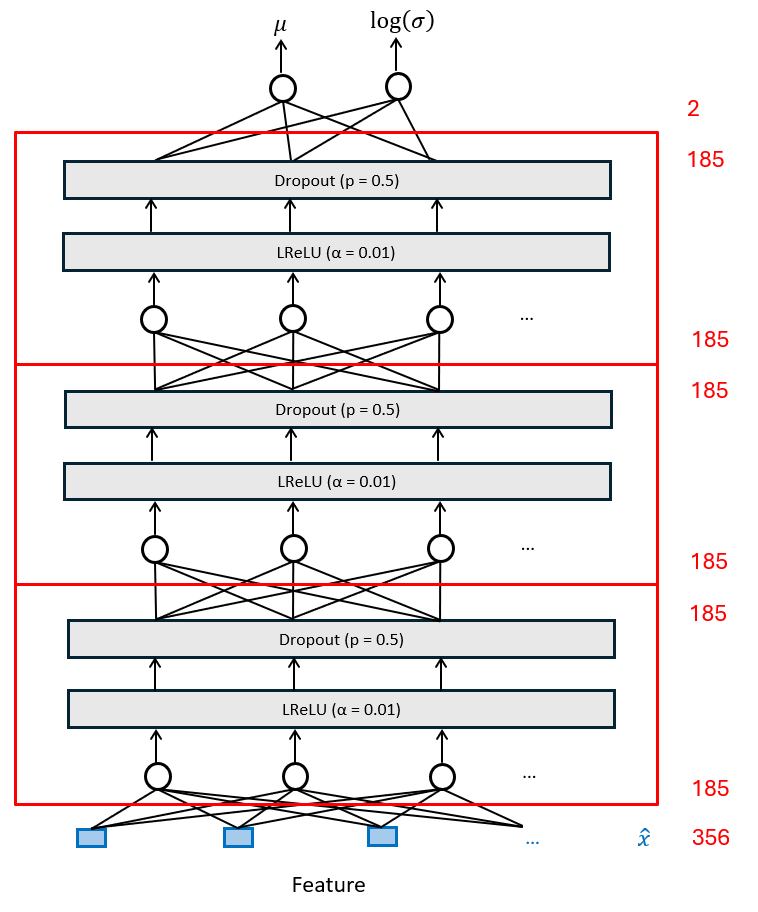
\includegraphics[width=0.7\textwidth]{feature.png}
    \caption{Feature-based model architecture}
    \label{fig:feature}
\end{figure}

\section{Audio-based Model}
Figure \ref{fig:audio} shows the architecture of the audio-based model. The wav2vec processing begins with the audio vector for each candidate described in \cite{graders}, which are 16kHz with duration 10-20 seconds. The data collator aggregates meta data (candidate number, attention masks), feeding vector to the wav2vec encoder, which creates contextualized embeddings for the tokens ($\mathcal{C}$). $\mathcal{C}$ is passed through two layers of 4 individual attention mechanisms. The output is concatenated to form the 3072-dimensional  token embeddings $\hat{x}$.

The token embeddings $\hat{x}$ is then passed through a fully connected DNN with a hidden layer, using the ReLU activation function and a dropout rate of 0.1. The output is a single scalar indicating the predicted score. As above, the red box and red number indicate the layers and the dimension change.

\begin{figure}[H]
    \centering
    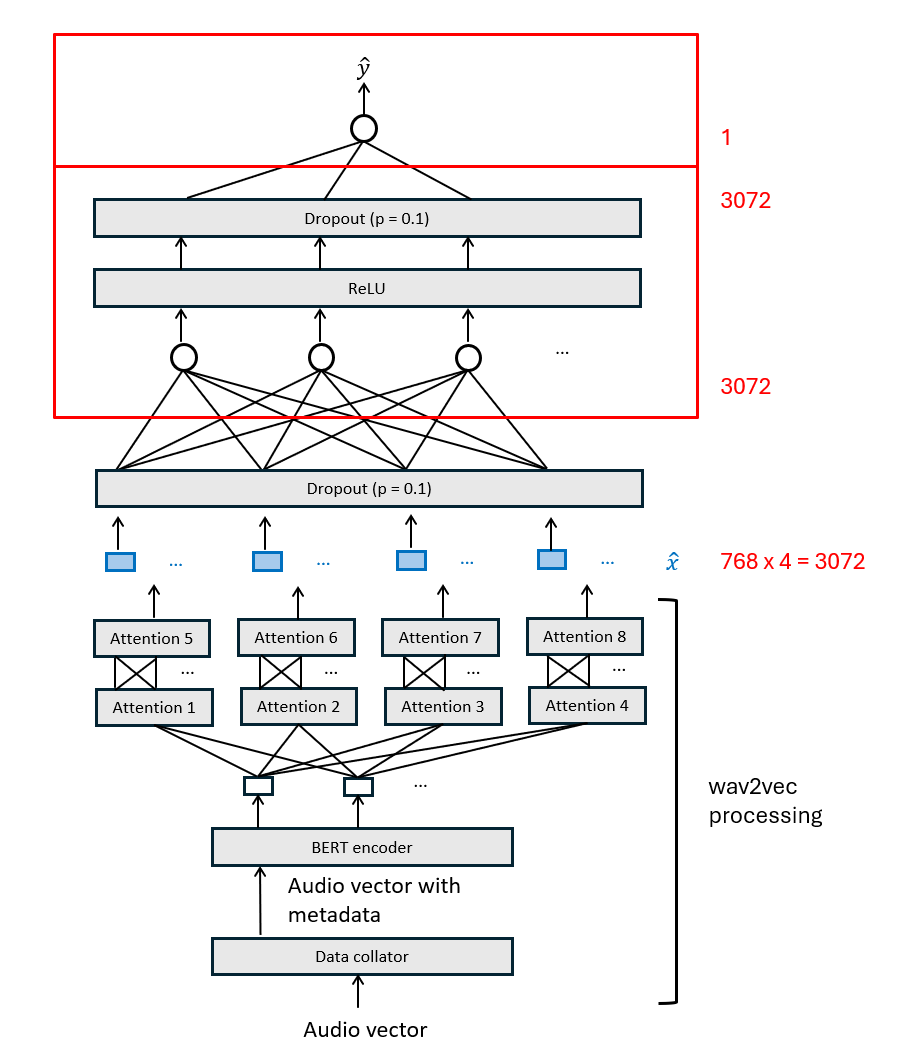
\includegraphics[width=0.7\textwidth]{audio.png}
    \caption{Audio-based model architecture}
    \label{fig:audio}
\end{figure}

\section{Summary}
This chapter describes the differences across the three types of models under investigation. Table \ref{tab:models} summarizes their key differences, including the input data, model type, activation function, dropout rate, and node numbers. Understanding these differences would be crucial for isolating factors that affect bias measurement.

\begin{table}[H]
    \centering
    \begin{tabular}{|c|c|c|c|}
        \hline
                                     & \textbf{Text-based}                                 & \textbf{Feature-based} & \textbf{Audio-based} \\ \hline
        \textbf{Intermediate Vector} & Text embeddings                                     & Feature vector         & Audio embeddings     \\ \hline
        \textbf{Model Type}          & DNN                                                 & DDN                    & DNN                  \\ \hline
        \textbf{Activation Function} & ReLU                                                & LReLU                  & ReLU                 \\ \hline
        \textbf{Dropout Rate}        & /                                                   & 0.5                    & 0.1                  \\ \hline
        \textbf{Node Numbers}        & $3072 \rightarrow 600 \rightarrow 20 \rightarrow 1$
                                     & \makecell[l]{
        $356 \rightarrow 185 \rightarrow$                                                                                                  \\
            $185 \rightarrow 185 \rightarrow 2$
        }
                                     & $3072 \rightarrow 3072 \rightarrow 1$                                                               \\ \hline
    \end{tabular}
    \caption{Summary of the three types of models under investigation}
    \label{tab:models}
\end{table}
